\documentclass[10pt,letterpaper]{report}

\usepackage{iftex}
\ifPDFTeX
    \usepackage[T1]{fontenc}
    \usepackage[utf8]{inputenc}
    \usepackage{helvet}
    \renewcommand{\familydefault}{\sfdefault}
\else
    \usepackage{fontspec}
    \setmainfont{Arial}
\fi
\usepackage[spanish]{babel}
\usepackage[top=20mm,bottom=20mm,left=25mm,right=25mm,letterpaper]{geometry}
\setlength{\parskip}{5pt}
\setlength{\parindent}{0pt}
\usepackage{hyperref}
\hypersetup{colorlinks=true,linkcolor=black,urlcolor=blue,citecolor=black}
\usepackage{graphicx}
\usepackage{float}
\usepackage{enumitem}
\usepackage{booktabs}
\usepackage{array}
\usepackage{tabularx}
\usepackage{longtable}
\usepackage{caption}
\usepackage{listings}
\usepackage{xcolor}
\usepackage{titlesec}
\usepackage{tocloft}
\usepackage{xurl}
\usepackage[most]{tcolorbox}

\counterwithout{figure}{chapter}
\counterwithout{table}{chapter}

% ── Code listing style ────────────────────────────────────────────────────────
\lstdefinestyle{cmd}{
  basicstyle=\ttfamily\small,
  backgroundcolor=\color{gray!10},
  frame=single,rulecolor=\color{gray!40},
  breaklines=true,
  columns=fullflexible,
  showstringspaces=false,
  xleftmargin=6pt,xrightmargin=6pt,
  aboveskip=6pt,belowskip=6pt
}
\lstdefinestyle{python}{
  language=Python,
  basicstyle=\ttfamily\small,
  backgroundcolor=\color{gray!10},
  frame=single,rulecolor=\color{gray!40},
  keywordstyle=\bfseries,
  breaklines=true,
  xleftmargin=6pt,xrightmargin=6pt,
  aboveskip=6pt,belowskip=6pt
}
\lstset{style=cmd}

% ── Alert box ─────────────────────────────────────────────────────────────────
\newtcolorbox{nota}{enhanced,breakable,
  colback=white,colframe=black!60,
  coltitle=black,fonttitle=\bfseries,title=Nota,
  boxrule=0.6pt,arc=2pt,left=6pt,right=6pt,top=3pt,bottom=3pt}
\newtcolorbox{alerta}{enhanced,breakable,
  colback=white,colframe=black,
  coltitle=black,fonttitle=\bfseries,title=Importante,
  boxrule=1pt,arc=2pt,left=6pt,right=6pt,top=3pt,bottom=3pt}

% ── Title formatting ─────────────────────────────────────────────────────────
\titleformat{\chapter}[block]{\large\bfseries}{}{0em}{}
\titlespacing*{\chapter}{0pt}{12pt}{6pt}
\titleformat{\section}[block]{\normalsize\bfseries}{\thesection}{1em}{}
\titleformat{\subsection}[block]{\normalsize\bfseries}{\thesubsection}{1em}{}
\setcounter{secnumdepth}{3}
\setcounter{tocdepth}{3}

\newcommand{\fechaentrega}{11 de junio de 2026}

% ===========================================================================
\begin{document}
% ===========================================================================

% ── PORTADA ─────────────────────────────────────────────────────────────────
\begin{titlepage}
\centering
\vspace*{1cm}

\includegraphics[width=4.2cm]{logo.png}\\[1.2cm]
{\large\textbf{Instituto Tecnológico y de Estudios Superiores de Monterrey}}\\[0.4cm]
{\normalsize Escuela de Ingeniería y Ciencias}\\[0.2cm]
{\normalsize Ingeniería en Ciencia de Datos y Matemáticas}\\[1.5cm]
{\large\textbf{Documentación de Desarrollo --- Gestor de Identidades v2.0}}\\[1.5cm]
{\normalsize\textbf{Casa Monarca --- Ayuda Humanitaria al Migrante A.B.P}}\\[1.5cm]
{\normalsize\textbf{Profesores:}}\\[0.3cm]
{\normalsize
Raúl Gómez Muñoz \quad Alberto Francisco Martínez Herrera\\
Pedro Leonel Olaya Trejos \quad Daniel Otero Fadul
}\\[1.5cm]
{\normalsize\textbf{Equipo 1 --- Grupo 602}}\\[0.3cm]
{\normalsize
Mariel Álvarez Salas \quad A01198828\\
Brisma Alvarez Valdez \quad A00839238\\
Emiliano Ruiz López \quad A01659693\\
Ana Sofia Nagao Alvarez \quad A01285034\\
Karen Aylen Estrada Ceferino \quad A00838403
}\\[1.5cm]
{Monterrey, Nuevo León. \fechaentrega}
\end{titlepage}

% ── ÍNDICES ──────────────────────────────────────────────────────────────────
\tableofcontents
\newpage
\listoftables
\newpage
\listoffigures
\newpage

% ===========================================================================
\chapter{Descripción General}
% ===========================================================================

\section{Propósito del sistema}

El sistema de Gestión de Identidades y Registro de Migrantes de Casa Monarca es una aplicación web interna desarrollada en Django cuyo propósito es doble:

\begin{enumerate}[leftmargin=*]
    \item \textbf{Módulo IAM (Identity \& Access Management):} controlar el ciclo de vida de los colaboradores de Casa Monarca. Emite y revoca certificados digitales X.509 para los niveles de mayor privilegio, lleva un registro de auditoría de todas las acciones y detecta intentos de acceso no autorizados.

    \item \textbf{Módulo de Registro de Migrantes:} gestionar expedientes de personas beneficiarias con cifrado AES-256 de los campos personales sensibles, firma ECDSA por expediente, un flujo de aprobación escalonado por nivel de acceso y herramientas para ejercer los derechos ARCO conforme a la LFPDPPP.
\end{enumerate}

\section{Alcance}

\textbf{Lo que el sistema hace:}
\begin{itemize}[leftmargin=*]
    \item Alta, baja, suspensión y revocación de colaboradores (Niveles 1--4).
    \item Emisión y revocación de certificados X.509 para Niveles 1 y 2.
    \item Onboarding con validación manual por parte del administrador.
    \item Registro de expedientes de migrantes con cifrado de datos personales.
    \item Firma ECDSA por expediente y cadena de auditoría criptográfica.
    \item Flujo de aprobación escalonado: Nivel 4 → 3 → 2 → 1.
    \item Gestión completa de los cuatro derechos ARCO con plazos legales calculados.
    \item Auditoría persistente e inalterable de todas las acciones del sistema.
    \item Recuperación de contraseña mediante pregunta de seguridad.
    \item Autenticación TOTP (MFA) opcional para Niveles 1 y 2.
\end{itemize}

\textbf{Limitaciones y fuera de alcance:}
\begin{itemize}[leftmargin=*]
    \item El sistema es una aplicación web interna; no hay API REST pública ni mobile app.
    \item No implementa notificaciones por correo electrónico en esta versión.
    \item No hay mecanismo de respaldo automático de base de datos (pendiente como mejora futura).
    \item La CA es autofirmada (self-signed); no está integrada con una autoridad certificadora externa.
    \item El servidor HostGator no soporta Java ni Docker, por lo que soluciones como Keycloak o step-ca quedan fuera del entorno de producción.
\end{itemize}

\section{Casos de uso principales}

\begin{table}[h!]
\centering
\caption{Casos de uso principales por módulo (elaboración propia).}
\label{tab:casosuso}
\begin{tabularx}{\textwidth}{l l X}
\toprule
\textbf{Módulo} & \textbf{Actor} & \textbf{Caso de uso} \\
\midrule
IAM & Admin (N1) & Alta/baja/revocación de colaborador; emisión/revocación de certificado \\
IAM & Colaborador & Onboarding; descarga de credenciales; recuperación de contraseña \\
IAM & Admin (N1) & Auditoría del sistema; gestión de certificados activos \\
Registros & N1/N2 & Crear/editar/eliminar registro de migrante directamente \\
Registros & N3/N4 & Solicitar creación o edición vía flujo de aprobación \\
Registros & N1/N2 & Aprobar, rechazar o ejecutar solicitudes del workflow \\
Registros & N3+ & Crear solicitud ARCO para un migrante \\
Registros & N2/N1 & Revisar, aprobar y ejecutar una solicitud ARCO \\
\bottomrule
\end{tabularx}
\end{table}

% ===========================================================================
\chapter{Arquitectura del Sistema}
% ===========================================================================

\section{Tipo de arquitectura}

El sistema sigue la arquitectura MVT (\textit{Model--View--Template}) de Django, una variante del patrón MVC donde:
\begin{itemize}[leftmargin=*]
    \item \textbf{Model:} define la estructura de datos y las reglas de negocio en \texttt{models.py}.
    \item \textbf{View:} contiene la lógica de cada petición HTTP en \texttt{views.py}; valida permisos, llama a los modelos y retorna respuestas.
    \item \textbf{Template:} las plantillas HTML en \texttt{templates/} renderizan la interfaz a partir del contexto enviado por las vistas.
\end{itemize}

La comunicación cliente--servidor es síncrona (peticiones HTTP convencionales); no se emplea AJAX salvo para marcar notificaciones como leídas. La capa criptográfica está aislada en el paquete \texttt{crypto\_core/}.

\section{Componentes principales}

\begin{table}[h!]
\centering
\caption{Componentes del sistema y su responsabilidad (elaboración propia).}
\label{tab:componentes}
\begin{tabularx}{\textwidth}{l X}
\toprule
\textbf{Componente} & \textbf{Responsabilidad} \\
\midrule
\texttt{casamonarca/} & Proyecto Django raíz: configuración, URL dispatcher principal \\
\texttt{iam/} & App IAM: modelos, vistas, URLs, lógica de onboarding y certificados \\
\texttt{registros/} & App registros: modelos CRUD, workflow, ARCO, tickets, cadena hash \\
\texttt{crypto\_core/} & Librería interna: cifrado AES-256, firmas ECDSA, CA, hashing, campos personalizados \\
\texttt{templates/} & Plantillas HTML organizadas por app \\
\texttt{static/} & CSS, JS e imágenes estáticas \\
\texttt{media/} & Archivos subidos por usuarios (IDs oficiales, documentos ARCO) \\
\texttt{tests/} & Suite de pruebas de integración criptográfica \\
\bottomrule
\end{tabularx}
\end{table}

\section{Diagrama general}

\begin{figure}[H]
\centering
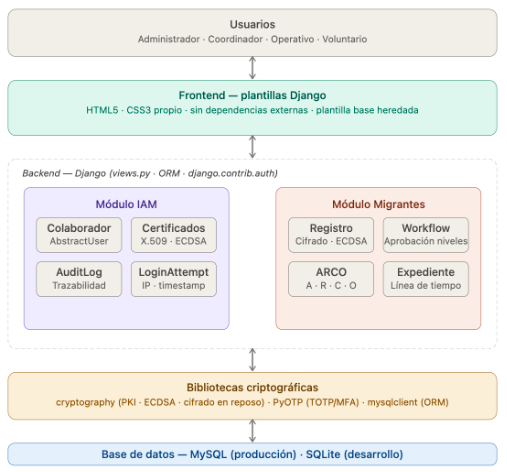
\includegraphics[width=0.88\textwidth]{arquitectura.png}
\caption{Diagrama de arquitectura del sistema. Generado con Claude (Anthropic, 2026).}
\label{fig:arquitectura}
\end{figure}

% ===========================================================================
\chapter{Stack Tecnológico}
% ===========================================================================

\begin{table}[h!]
\centering
\caption{Stack tecnológico completo (elaboración propia).}
\label{tab:stack}
\begin{tabularx}{\textwidth}{l l X}
\toprule
\textbf{Categoría} & \textbf{Tecnología} & \textbf{Versión / Uso} \\
\midrule
Lenguaje & Python & 3.10 o superior \\
Framework web & Django & $\geq$5.0, $<$7.0 \\
Base de datos (prod) & MySQL & 8.0+ vía \texttt{PyMySQL$\geq$1.0} \\
Base de datos (dev) & SQLite & Incluida en Python; sin configuración \\
Criptografía & \texttt{cryptography} & $\geq$41.0 (AES-256-GCM, ECDSA, X.509) \\
MFA & \texttt{pyotp} & $\geq$2.0 (TOTP RFC 6238) \\
JWT & \texttt{PyJWT} & $\geq$2.8.0 (tokens auxiliares) \\
Variables de entorno & \texttt{python-dotenv} & $\geq$1.0 \\
Pruebas & \texttt{pytest} + \texttt{pytest-django} & $\geq$7.0 y $\geq$4.5 \\
Teléfonos & \texttt{phonenumbers} & Última estable \\
Servidor producción & Gunicorn + nginx & Recomendado para HostGator \\
\bottomrule
\end{tabularx}
\end{table}

% ===========================================================================
\chapter{Estructura del Proyecto}
% ===========================================================================

\section{Organización de carpetas}

\begin{lstlisting}
CriptoReto/
|-- casamonarca/          # Proyecto Django raiz
|   |-- settings.py       # Configuracion central
|   |-- urls.py           # URL dispatcher principal
|   `-- wsgi.py / asgi.py
|-- iam/                  # App: gestion de identidades
|   |-- models.py         # Collaborator, UserCertificate, AuditLog, LoginAttempt
|   |-- views.py          # Vistas de login, onboarding, certificados
|   |-- urls.py           # 42 rutas del modulo IAM
|   `-- management/commands/  # Comandos personalizados
|-- registros/            # App: registros de migrantes
|   |-- models.py         # 12 modelos (MigrantRegistration, WorkflowRequest, etc.)
|   |-- views.py          # Vistas CRUD, workflow, ARCO
|   |-- urls.py           # 50+ rutas del modulo registros
|   `-- workflow.py       # Logica de escalacion del flujo de aprobacion
|-- crypto_core/          # Libreria criptografica interna
|   |-- encryption.py     # AES-256-GCM (EncryptionService)
|   |-- signatures.py     # ECDSA con SECP256K1
|   |-- ca.py             # Autoridad Certificadora interna
|   |-- certificates.py   # Emision y verificacion de certificados X.509
|   |-- fields.py         # EncryptedTextField, EncryptedDateField
|   `-- hashing.py        # SHA-256 y utilidades de hash
|-- templates/            # Plantillas HTML
|   |-- iam/              # Pantallas del modulo IAM
|   |-- registros/        # Pantallas del modulo registros
|   `-- partials/         # Componentes reutilizables (base, navbar, etc.)
|-- static/               # CSS, JS, imagenes estaticas
|-- media/                # Archivos subidos (IDs oficiales, PDFs ARCO)
|   |-- official_ids/
|   |-- arco_docs/
|   `-- arco_exports/
|-- tests/
|   `-- test_crypto_integration.py
|-- scripts/              # Scripts auxiliares (seed, migraciones iniciales)
|-- seed.py               # Poblar BD con datos de prueba
|-- requirements.txt
`-- manage.py
\end{lstlisting}

\section{Descripción de módulos}

\subsection{iam}
Gestiona el ciclo de vida de los colaboradores. Contiene los modelos \texttt{Area}, \texttt{Collaborator} (extiende \texttt{AbstractUser}), \texttt{UserCertificate}, \texttt{CertificateAuditLog}, \texttt{AuditLog} y \texttt{LoginAttempt}. La lógica de control de acceso está encapsulada en métodos de instancia del modelo \texttt{Collaborator} (\texttt{can\_view}, \texttt{can\_edit}, \texttt{can\_issue\_certificate}, etc.).

\subsection{registros}
Gestiona los expedientes de migrantes y los flujos de aprobación. Contiene 12 modelos: \texttt{MigrantRegistration}, \texttt{MigrantRegistrationSignature}, \texttt{ActionSignature}, \texttt{BatchSignSession}, \texttt{WorkflowRequest}, \texttt{ApprovalStep}, \texttt{Ticket}, \texttt{ArcoRequest}, \texttt{ArcoTicket}, \texttt{Notification}, \texttt{RegistrationEvent} y \texttt{SignedFlowLog}. El archivo \texttt{workflow.py} encapsula las reglas de escalación.

\subsection{crypto\_core}
Librería criptográfica interna que ningún código externo debería reimplementar. Expone:
\begin{itemize}[leftmargin=*]
    \item \texttt{EncryptionService}: cifrado y descifrado AES-256-GCM.
    \item \texttt{ECDSASigner}: firma y verificación ECDSA sobre \texttt{secp256k1}.
    \item \texttt{CertificateAuthority}: generación y verificación de certificados X.509.
    \item \texttt{EncryptedTextField} / \texttt{EncryptedDateField}: campos Django con cifrado transparente en el ORM.
    \item \texttt{sha256\_hex}: función auxiliar SHA-256.
\end{itemize}

% ===========================================================================
\chapter{Configuración del Entorno}
% ===========================================================================

\section{Requisitos de versión}

\begin{table}[h!]
\centering
\caption{Requisitos del entorno de desarrollo y producción (elaboración propia).}
\label{tab:requisitos}
\begin{tabularx}{\textwidth}{l l X}
\toprule
\textbf{Componente} & \textbf{Versión mínima} & \textbf{Notas} \\
\midrule
Python & 3.10 & Se recomienda 3.11 o 3.12 \\
pip & 23.0+ & Incluido con Python \\
MySQL & 8.0 & Solo en producción; SQLite en desarrollo \\
Git & 2.30+ & Para clonar el repositorio \\
Sistema operativo & macOS 12 / Ubuntu 20.04 / Windows 10+WSL & HostGator usa cPanel con Python \\
\bottomrule
\end{tabularx}
\end{table}

\section{Variables de entorno}

El sistema lee variables de entorno mediante \texttt{python-dotenv}. En desarrollo se utiliza un archivo \texttt{.env} en la raíz del proyecto. En producción deben configurarse en el entorno del servidor (cPanel $\to$ Variables de entorno).

\begin{table}[H]
\centering
\caption{Variables de entorno del sistema (elaboración propia).}
\label{tab:envvars}
\begin{tabularx}{\textwidth}{l l X}
\toprule
\textbf{Variable} & \textbf{Obligatoria} & \textbf{Descripción} \\
\midrule
\texttt{SECRET\_KEY} & Sí (prod) & Clave secreta de Django. Generar con \texttt{django-admin startproject} o \texttt{secrets.token\_urlsafe(50)}. \\
\texttt{DEBUG} & No & \texttt{True} en desarrollo, \texttt{False} en producción. \\
\texttt{ALLOWED\_HOSTS} & Sí (prod) & Lista de dominios permitidos, p.ej. \texttt{casamonarca.org}. \\
\texttt{MYSQL\_DATABASE} & Sí (prod) & Nombre de la base de datos MySQL. Si no está definida, usa SQLite. \\
\texttt{MYSQL\_USER} & Prod & Usuario MySQL (\textit{default}: \texttt{casamonarca\_user}). \\
\texttt{MYSQL\_PASSWORD} & Prod & Contraseña MySQL. \\
\texttt{MYSQL\_HOST} & Prod & Host MySQL (\textit{default}: \texttt{127.0.0.1}). \\
\texttt{MYSQL\_PORT} & No & Puerto MySQL (\textit{default}: \texttt{3306}). \\
\texttt{CERT\_ENCRYPTION\_KEY} & Sí (prod) & Clave base64 de 32 bytes para cifrar datos de certificados. En \texttt{DEBUG=True} se deriva de \texttt{SECRET\_KEY}. \\
\texttt{CERT\_ISSUER\_NAME} & No & Nombre del emisor X.509 (\textit{default}: \texttt{Casa Monarca IAM}). \\
\texttt{CERT\_EXPIRATION\_DAYS} & No & Vigencia de certificados en días (\textit{default}: \texttt{365}). \\
\texttt{CERT\_PRIVATE\_KEY\_PATH} & Sí (prod) & Ruta a la clave privada PEM de la CA interna. \\
\texttt{ECC\_PRIVATE\_KEY\_PATH} & Sí (prod) & Ruta a la clave ECC PEM utilizada para firmas del servidor. \\
\bottomrule
\end{tabularx}
\end{table}

\section{Archivos de configuración}

\textbf{\texttt{casamonarca/settings.py}} --- configuración central de Django. No editar directamente en producción; usar variables de entorno.

\textbf{\texttt{.env}} (no subir al repositorio) --- ejemplo mínimo para desarrollo:
\begin{lstlisting}
SECRET_KEY=django-dev-only-key-change-in-production
DEBUG=True
# Dejar MYSQL_DATABASE sin definir para usar SQLite en desarrollo
# CERT_ENCRYPTION_KEY se deriva automaticamente en DEBUG=True
CERT_ISSUER_NAME=Casa Monarca IAM (Dev)
CERT_EXPIRATION_DAYS=365
ECC_PRIVATE_KEY_PATH=./ecc_signing_key.pem
\end{lstlisting}

\textbf{\texttt{requirements.txt}} --- dependencias pinadas por versión mínima:
\begin{lstlisting}
Django>=5.0,<7.0
PyMySQL>=1.0
pyotp>=2.0
cryptography>=41.0
PyJWT>=2.8.0
python-dotenv>=1.0
pytest>=7.0
pytest-django>=4.5
phonenumbers
\end{lstlisting}

% ===========================================================================
\chapter{Instalación y Ejecución}
% ===========================================================================

\section{Pasos para levantar el sistema}

\textbf{Paso 1 — Clonar el repositorio:}
\begin{lstlisting}
git clone https://github.com/[organizacion]/Casa-Monarca-Criptografia.git
cd Casa-Monarca-Criptografia/CriptoReto
\end{lstlisting}

\textbf{Paso 2 — Crear y activar el entorno virtual:}
\begin{lstlisting}
python -m venv venv
source venv/bin/activate          # macOS / Linux
# venv\Scripts\activate           # Windows
\end{lstlisting}

\textbf{Paso 3 — Instalar dependencias:}
\begin{lstlisting}
pip install -r requirements.txt
\end{lstlisting}

\textbf{Paso 4 — Configurar variables de entorno:}
\begin{lstlisting}
cp .env.example .env   # si existe, o crear manualmente
# Editar .env con los valores reales
\end{lstlisting}

\textbf{Paso 5 — Aplicar migraciones:}
\begin{lstlisting}
python manage.py migrate
\end{lstlisting}

\textbf{Paso 6 — Crear administrador inicial:}
\begin{lstlisting}
python manage.py createsuperuser
\end{lstlisting}

\textbf{Paso 7 — (Opcional) Cargar datos semilla:}
\begin{lstlisting}
python seed.py
\end{lstlisting}

\textbf{Paso 8 — Iniciar el servidor de desarrollo:}
\begin{lstlisting}
python manage.py runserver
\end{lstlisting}
El sistema queda disponible en \url{http://127.0.0.1:8000}.

\section{Comandos principales}

\begin{table}[H]
\centering
\caption{Comandos de gestión más usados (elaboración propia).}
\label{tab:comandos}
\begin{tabularx}{\textwidth}{l X}
\toprule
\textbf{Comando} & \textbf{Descripción} \\
\midrule
\texttt{python manage.py migrate} & Aplica migraciones pendientes \\
\texttt{python manage.py makemigrations} & Genera nuevas migraciones a partir de cambios en modelos \\
\texttt{python manage.py createsuperuser} & Crea el primer administrador (Nivel 1) \\
\texttt{python manage.py collectstatic} & Reúne estáticos para producción \\
\texttt{python manage.py shell} & REPL de Django con todos los modelos cargados \\
\texttt{pytest} & Ejecuta la suite completa de pruebas \\
\texttt{pytest tests/ -v} & Pruebas con salida detallada \\
\bottomrule
\end{tabularx}
\end{table}

% ===========================================================================
\chapter{Base de Datos}
% ===========================================================================

\section{Modelo de datos}

El sistema tiene 18 tablas distribuidas en dos aplicaciones Django. Los nombres en la base de datos siguen la convención \texttt{<app>\_<model>} (p.ej. \texttt{iam\_collaborator}, \texttt{registros\_migrantregistration}).

\section{Tablas principales}

\begin{table}[H]
\centering
\caption{Tablas principales del sistema (elaboración propia).}
\label{tab:tablas}
\begin{tabularx}{\textwidth}{l l X}
\toprule
\textbf{Tabla} & \textbf{App} & \textbf{Descripción} \\
\midrule
\texttt{iam\_collaborator} & iam & Extiende \texttt{auth\_user}. Contiene nivel de acceso, estado de onboarding, campos de revocación, TOTP y pregunta de seguridad. \\
\texttt{iam\_usercertificate} & iam & Certificado X.509 de un colaborador. Relación 1:1 con \texttt{Collaborator}. Almacena datos cifrados, huella digital, estado y fechas del ciclo de vida. \\
\texttt{iam\_certificateauditlog} & iam & Registro inmutable de cada cambio de estado de un certificado. No permite UPDATE ni DELETE. \\
\texttt{iam\_auditlog} & iam & Bitácora general del sistema: actor, objetivo, acción, timestamp. \\
\texttt{iam\_loginattempt} & iam & Registro de cada intento de inicio de sesión con IP y resultado. \\
\texttt{registros\_migrantregistration} & registros & Expediente del migrante. Campos PII (nombre, apellidos, fecha nacimiento, teléfono, país) cifrados con AES-256-GCM. \\
\texttt{registros\_migrantregistrationsignature} & registros & Firma ECDSA del expediente. Relación 1:1. Guarda $(r, s)$, clave pública, curva, firmante. \\
\texttt{registros\_actionsignature} & registros & Firma de cualquier acción del sistema. Encadenada por \texttt{prev\_chain\_hash} (SHA-256). \\
\texttt{registros\_workflowrequest} & registros & Solicitud de creación/edición/eliminación que requiere aprobación jerárquica. \\
\texttt{registros\_approvalstep} & registros & Decisión individual dentro de un \texttt{WorkflowRequest}. Append-only con cadena de hash. \\
\texttt{registros\_arcorequest} & registros & Solicitud ARCO formal con plazo legal y documentos adjuntos. \\
\texttt{registros\_arcoticket} & registros & Flujo de autorización ARCO-específico (coordinador → administrador). \\
\texttt{registros\_ticket} & registros & Ticket genérico creado automáticamente al crear un registro o workflow. \\
\texttt{registros\_registrationevent} & registros & Bitácora por expediente: consultas, ediciones, consentimientos, ARCO. \\
\texttt{registros\_signedflowlog} & registros & Log inmutable de acciones irreversibles firmadas con X.509. No permite UPDATE ni DELETE. \\
\texttt{registros\_notification} & registros & Notificación interna enviada al responsable de un workflow o ARCO. \\
\bottomrule
\end{tabularx}
\end{table}

\section{Relaciones clave}

\begin{itemize}[leftmargin=*]
    \item \texttt{Collaborator} (1) $\leftrightarrow$ (0..1) \texttt{UserCertificate} — un colaborador puede tener un certificado activo o ninguno.
    \item \texttt{UserCertificate} (1) $\to$ (N) \texttt{CertificateAuditLog} — cada cambio de estado genera un registro append-only.
    \item \texttt{MigrantRegistration} (1) $\leftrightarrow$ (1) \texttt{MigrantRegistrationSignature} — todo expediente tiene exactamente una firma ECDSA.
    \item \texttt{MigrantRegistration} (1) $\to$ (N) \texttt{WorkflowRequest} — puede tener múltiples solicitudes de cambio a lo largo del tiempo.
    \item \texttt{WorkflowRequest} (1) $\to$ (N) \texttt{ApprovalStep} — cada decisión de cada aprobador queda registrada.
    \item \texttt{ArcoRequest} (1) $\leftrightarrow$ (1) \texttt{ArcoTicket} — cada solicitud ARCO tiene su ticket de seguimiento.
    \item \texttt{ActionSignature} — cadena encadenada mediante \texttt{prev\_chain\_hash}; el primer registro tiene \texttt{prev\_chain\_hash=""}.
\end{itemize}

% ===========================================================================
\chapter{API / Interfaces (Rutas URL)}
% ===========================================================================

\section{Módulo IAM}

Prefijo base: \texttt{/iam/} (definido en \texttt{casamonarca/urls.py}).

\begin{longtable}{l l p{4.5cm}}
\caption{Rutas del módulo IAM (elaboración propia).}
\label{tab:routes_iam}\\
\toprule
\textbf{Ruta} & \textbf{Métodos} & \textbf{Descripción} \\
\midrule
\endfirsthead
\toprule
\textbf{Ruta} & \textbf{Métodos} & \textbf{Descripción} \\
\midrule
\endhead
\bottomrule
\endfoot
\texttt{/iam/login/} & GET, POST & Formulario de inicio de sesión con \texttt{.cert}/\texttt{.key} para N1--N2 \\
\texttt{/iam/logout/} & POST & Cierre de sesión \\
\texttt{/iam/} & GET & Dashboard con estadísticas del IAM \\
\texttt{/iam/users/add/} & GET, POST & Crear nuevo colaborador (solo Admin) \\
\texttt{/iam/users/<pk>/} & GET & Detalle de colaborador \\
\texttt{/iam/users/<pk>/edit/} & GET, POST & Editar colaborador \\
\texttt{/iam/users/<pk>/toggle/} & POST & Activar/desactivar cuenta \\
\texttt{/iam/users/<pk>/revoke/} & POST & Revocar acceso \\
\texttt{/iam/users/<pk>/delete/} & POST & Eliminación lógica \\
\texttt{/iam/users/<pk>/certificate/issue/} & GET, POST & Emitir certificado X.509 \\
\texttt{/iam/users/<pk>/certificate/validate/} & GET & Verificar validez del certificado \\
\texttt{/iam/users/<pk>/certificate/revoke/} & POST & Revocar certificado \\
\texttt{/iam/onboarding/} & GET, POST & Formulario de onboarding del propio usuario \\
\texttt{/iam/onboarding/download/} & GET & Descargar \texttt{.cert} \\
\texttt{/iam/onboarding/download/key/} & GET & Descargar \texttt{.key} \\
\texttt{/iam/onboarding/pending/} & GET & Lista de onboardings pendientes (Admin) \\
\texttt{/iam/users/<pk>/onboarding/approve/} & POST & Aprobar onboarding \\
\texttt{/iam/audit/} & GET & Visor de auditoría con filtros \\
\texttt{/iam/certificados/} & GET & Gestión de certificados (Admin) \\
\texttt{/iam/certificados/<id>/suspender/} & POST & Suspender certificado \\
\texttt{/iam/certificados/<id>/reactivar/} & POST & Reactivar certificado suspendido \\
\texttt{/iam/certificados/<id>/baja/} & POST & Dar de baja un certificado \\
\texttt{/iam/recovery/} & GET, POST & Solicitar recuperación de contraseña \\
\texttt{/iam/password/change/} & GET, POST & Cambio de contraseña autenticado \\
\texttt{/iam/api/user-role/} & GET & JSON con nivel y tipo del usuario en sesión \\
\end{longtable}

\section{Módulo Registros}

Prefijo base: \texttt{/registros/}.

\begin{longtable}{l l p{4.5cm}}
\caption{Rutas del módulo Registros (elaboración propia).}
\label{tab:routes_reg}\\
\toprule
\textbf{Ruta} & \textbf{Métodos} & \textbf{Descripción} \\
\midrule
\endfirsthead
\toprule
\textbf{Ruta} & \textbf{Métodos} & \textbf{Descripción} \\
\midrule
\endhead
\bottomrule
\endfoot
\texttt{/registros/} & GET & Listado de expedientes activos \\
\texttt{/registros/nuevo/} & GET, POST & Formulario de nuevo registro \\
\texttt{/registros/nuevo/revisar/} & GET, POST & Revisión y confirmación con firma \\
\texttt{/registros/<pk>/} & GET & Detalle del expediente \\
\texttt{/registros/<pk>/editar/} & GET, POST & Editar registro (N1/N2 directo) \\
\texttt{/registros/<pk>/eliminar/} & POST & Eliminación lógica (N1) \\
\texttt{/registros/<pk>/expediente/} & GET & Línea de tiempo del expediente \\
\texttt{/registros/<pk>/verificar/} & GET & Verificar firma ECDSA del registro \\
\texttt{/registros/workflow/} & GET & Listado de solicitudes de cambio \\
\texttt{/registros/workflow/<pk>/decide/} & POST & Aprobar o rechazar solicitud \\
\texttt{/registros/workflow/<pk>/execute/} & POST & Ejecutar solicitud aprobada \\
\texttt{/registros/arco/} & GET & Listado de solicitudes ARCO \\
\texttt{/registros/<pk>/arco/nueva/} & GET, POST & Nueva solicitud ARCO para un registro \\
\texttt{/registros/arco/<pk>/} & GET & Detalle de solicitud ARCO \\
\texttt{/registros/arco/<pk>/ejecutar/} & POST & Ejecutar solicitud ARCO \\
\texttt{/registros/cadena/} & GET & Visor de la cadena de auditoría criptográfica \\
\texttt{/registros/tickets/} & GET & Listado de tickets del sistema \\
\end{longtable}

\section{Ejemplo de uso: crear registro vía vistas}

\begin{lstlisting}[style=python]
# Fragmento simplificado de views.py en registros/
from crypto_core.signatures import ECDSASigner
from crypto_core.hashing import sha256_hex

def registro_review(request):
    # 1. Recuperar datos del formulario (guardados en sesion)
    data = request.session.get('registro_draft')
    # 2. Firmar con la clave del usuario autenticado
    payload = json.dumps(data, sort_keys=True)
    msg_hash = sha256_hex(payload.encode())
    signer = ECDSASigner(private_key_pem=request.session['private_key_pem'])
    r, s = signer.sign(payload.encode())
    # 3. Crear el registro y su firma
    reg = MigrantRegistration.objects.create(**data, created_by=request.user)
    MigrantRegistrationSignature.objects.create(
        registration=reg, message_hash=msg_hash,
        signature_r=str(r), signature_s=str(s),
        public_key=signer.public_key_pem(), curve_name='secp256k1',
        signed_by=request.user, signed_by_role=request.user.access_level,
    )
\end{lstlisting}

% ===========================================================================
\chapter{Flujos y Lógica de Negocio}
% ===========================================================================

\section{Flujo de autenticación (login)}

\begin{enumerate}[leftmargin=*]
    \item El usuario envía \texttt{username} + \texttt{password} + (para N1/N2) los archivos \texttt{.cert} y \texttt{.key}.
    \item El sistema verifica el límite de intentos fallidos: si hay 5 o más en los últimos 15 minutos (\texttt{LoginAttempt.is\_blocked}), rechaza con código \texttt{429}.
    \item Autenticación Django con \texttt{authenticate()}. Si falla, registra un \texttt{LoginAttempt(successful=False)}.
    \item Si el usuario tiene \texttt{is\_revoked=True} o \texttt{is\_deleted=True}: error ``Cuenta inactiva o revocada''.
    \item Si el \texttt{onboarding\_status} es \texttt{pending}: redirige a \texttt{/iam/onboarding/}.
    \item Para N1/N2: verifica que el \texttt{.cert} presentado coincide con el \texttt{fingerprint} almacenado en \texttt{UserCertificate} y que el certificado no está revocado ni expirado.
    \item Si el usuario tiene MFA activo: solicita el código TOTP; se verifica con \texttt{pyotp.TOTP.verify}.
    \item Sesión iniciada; registra \texttt{LoginAttempt(successful=True)} y entrada en \texttt{AuditLog}.
\end{enumerate}

\section{Flujo de onboarding de nuevo colaborador}

\begin{enumerate}[leftmargin=*]
    \item Admin crea el colaborador con contraseña temporal (\texttt{onboarding\_status='pending'}).
    \item El colaborador ingresa y completa el formulario de onboarding: datos personales, ID oficial, pregunta de seguridad.
    \item El estado cambia a \texttt{submitted}; el Admin visualiza la solicitud en \texttt{/iam/onboarding/pending/}.
    \item Admin aprueba: estado → \texttt{approved}; si nivel $\leq$ 2, el sistema emite automáticamente el certificado X.509 y el par de claves.
    \item El colaborador descarga sus archivos \texttt{.cert} y \texttt{.key}; los campos \texttt{cert\_file\_downloaded} y \texttt{key\_file\_downloaded} se marcan en \texttt{True}.
    \item En el siguiente login el colaborador presenta sus credenciales digitales junto con usuario y contraseña.
\end{enumerate}

\section{Flujo del workflow de aprobación}

\begin{table}[H]
\centering
\caption{Reglas de escalación por tipo de acción (elaboración propia).}
\label{tab:escalacion}
\begin{tabularx}{\textwidth}{l l X}
\toprule
\textbf{Tipo de acción} & \textbf{Solicitante} & \textbf{Cadena de aprobación} \\
\midrule
Crear registro & N4 & N3 revisa → N2 aprueba → N1 ejecuta \\
Actualizar registro & N3/N4 & N2 aprueba → N1 ejecuta \\
Eliminar registro & Cualquiera & Escala hasta N1 \\
ARCO Acceso/Oposición & N3+ & N2 autoriza → N1 ejecuta \\
ARCO Rectificación & N3+ & N2 ejecuta \\
ARCO Cancelación & Cualquiera & N1 ejecuta únicamente \\
\bottomrule
\end{tabularx}
\end{table}

Los estados del workflow son: \texttt{submitted} → \texttt{pending\_review} → \texttt{escalated} → \texttt{approved} → \texttt{signed} → \texttt{executed} (o \texttt{rejected} en cualquier punto). Cada transición de estado requiere la firma digital del actor.

\section{Reglas importantes}

\begin{itemize}[leftmargin=*]
    \item \textbf{Inmutabilidad:} los modelos \texttt{CertificateAuditLog}, \texttt{SignedFlowLog} y los \texttt{ApprovalStep} no permiten UPDATE ni DELETE a nivel de modelo Python (el método \texttt{save()} lanza \texttt{PermissionError} si ya tiene PK).
    \item \textbf{Cifrado transparente:} los campos declarados como \texttt{EncryptedTextField} o \texttt{EncryptedDateField} se cifran automáticamente al escribir en la BD y se descifran al leer. El código de las vistas trabaja siempre con valores en claro.
    \item \textbf{Eliminación lógica:} ningún expediente se borra físicamente de la BD. El campo \texttt{is\_deleted=True} oculta el registro del listado público; solo el administrador puede verlo en \texttt{/registros/eliminados/}.
    \item \textbf{Plazo ARCO:} al crear un \texttt{ArcoRequest}, el sistema calcula automáticamente \texttt{legal\_deadline = fecha\_recepción + 20 días hábiles}.
    \item \textbf{Identificadores únicos:} \texttt{Collaborator.internal\_id} sigue el patrón \texttt{CM-XXXXXXXX}; \texttt{MigrantRegistration.internal\_id} sigue \texttt{MIG-XXXXXXXX}; \texttt{ArcoRequest.case\_id} sigue \texttt{ARCO-XXXXXXXX}. Se generan en \texttt{save()} si están vacíos.
\end{itemize}

% ===========================================================================
\chapter{Ejemplos de Uso}
% ===========================================================================

\section{Crear un colaborador desde código}

\begin{lstlisting}[style=python]
from iam.models import Collaborator, Area

area = Area.objects.get(slug='humanitaria')
colaborador = Collaborator.objects.create_user(
    username='jdoe',
    email='jdoe@casamonarca.org',
    password='TempPass2026!',
    access_level=3,
    area=area,
    role='Operativo Humanitario',
)
# El internal_id se asigna automaticamente en save()
print(colaborador.internal_id)  # CM-A1B2C3D4
\end{lstlisting}

\section{Emitir un certificado X.509}

\begin{lstlisting}[style=python]
from crypto_core.ca import CertificateAuthority
from iam.models import UserCertificate

ca = CertificateAuthority()
cert_pem, key_pem, fingerprint = ca.issue_certificate(
    subject_name=colaborador.get_full_name(),
    days_valid=365,
)
UserCertificate.objects.create(
    collaborator=colaborador,
    certificate_data=cert_pem,
    key_data=key_pem,  # cifrado con CERT_ENCRYPTION_KEY
    fingerprint=fingerprint,
    expires_at=timezone.now() + timedelta(days=365),
    issued_by=admin_user,
)
\end{lstlisting}

\section{Firmar y verificar un expediente}

\begin{lstlisting}[style=python]
from crypto_core.signatures import ECDSASigner
import json

# Firma
payload = json.dumps({'internal_id': 'MIG-00000001',
                      'first_name': 'Juan'}, sort_keys=True)
signer = ECDSASigner(private_key_pem=key_pem)
r, s = signer.sign(payload.encode())

# Verificacion
verifier = ECDSASigner(public_key_pem=signer.public_key_pem())
valid = verifier.verify(payload.encode(), r, s)
print(valid)  # True
\end{lstlisting}

\section{Consultar el estado de la cadena de auditoría}

\begin{lstlisting}[style=python]
from registros.models import ActionSignature

# Verificar que la cadena no ha sido manipulada
entries = ActionSignature.objects.order_by('chain_position')
prev_hash = ''
for entry in entries:
    if entry.prev_chain_hash != prev_hash:
        print(f"CADENA ROTA en posicion {entry.chain_position}")
        break
    prev_hash = entry.chain_hash()
else:
    print("Cadena integra.")
\end{lstlisting}

% ===========================================================================
\chapter{Manejo de Errores}
% ===========================================================================

\section{Estrategia de errores}

El sistema sigue la estrategia de Django para el manejo de errores HTTP:
\begin{itemize}[leftmargin=*]
    \item \textbf{403 Forbidden:} cuando un usuario intenta acceder a una vista para la que no tiene el nivel de acceso requerido. Django devuelve la plantilla \texttt{403.html}.
    \item \textbf{404 Not Found:} cuando se solicita un objeto con un ID que no existe (\texttt{get\_object\_or\_404}).
    \item \textbf{500 Internal Server Error:} errores no capturados. En producción (\texttt{DEBUG=False}), Django registra el error y muestra una página genérica.
\end{itemize}

Para errores de negocio (formularios inválidos, firma incorrecta, certificado expirado), las vistas retornan el formulario con mensajes de error explícitos a través del sistema de mensajes de Django (\texttt{messages.error}).

\section{Mensajes comunes}

\begin{table}[H]
\centering
\caption{Mensajes de error frecuentes y su causa (elaboración propia).}
\label{tab:errores}
\begin{tabularx}{\textwidth}{l X X}
\toprule
\textbf{Mensaje} & \textbf{Causa} & \textbf{Acción} \\
\midrule
\textit{``Usuario o contraseña incorrectos''} & Credenciales inválidas & Verificar datos; revisar \texttt{LoginAttempt} \\
\textit{``Cuenta inactiva o revocada''} & \texttt{is\_revoked=True} o \texttt{is\_deleted=True} & Contactar al administrador \\
\textit{``Certificado inválido o expirado''} & \texttt{UserCertificate} revocado o \texttt{expires\_at} pasado & Solicitar renovación \\
\textit{``Debes aceptar el Aviso de Privacidad''} & \texttt{data\_consent=False} en el formulario & Marcar el campo de consentimiento \\
\textit{``Los menores no pueden superar el tamaño del grupo''} & Validación de consistencia del registro & Revisar los campos de grupo y menores \\
\texttt{CERT\_ENCRYPTION\_KEY must be set in production} & Variable de entorno faltante & Configurar \texttt{CERT\_ENCRYPTION\_KEY} en producción \\
\bottomrule
\end{tabularx}
\end{table}

\section{Registro (logs)}

\begin{itemize}[leftmargin=*]
    \item \textbf{\texttt{AuditLog}:} registra todas las acciones IAM con \texttt{actor}, \texttt{target}, \texttt{action} y \texttt{created\_at}. Visible en \texttt{/iam/audit/}.
    \item \textbf{\texttt{LoginAttempt}:} registra cada intento de inicio de sesión con IP, usuario y resultado. Permite detectar fuerza bruta.
    \item \textbf{\texttt{RegistrationEvent}:} bitácora por expediente (consultas, ediciones, eventos ARCO). Visible en \texttt{/registros/<pk>/expediente/}.
    \item \textbf{\texttt{CertificateAuditLog}:} historial de cambios de estado de cada certificado. Append-only.
    \item En producción, Django escribe errores no capturados en el log del servidor (configurado en \texttt{LOGGING} dentro de \texttt{settings.py}).
\end{itemize}

% ===========================================================================
\chapter{Pruebas}
% ===========================================================================

\section{Tipos de tests}

El proyecto incluye pruebas de integración criptográfica ubicadas en \texttt{tests/test\_crypto\_integration.py}. Estas pruebas validan:
\begin{itemize}[leftmargin=*]
    \item Cifrado y descifrado simétrico con \texttt{EncryptionService} (AES-256-GCM).
    \item Generación, firma y verificación ECDSA con \texttt{ECDSASigner}.
    \item Emisión y verificación de certificados X.509 con \texttt{CertificateAuthority}.
    \item Integridad de la cadena de auditoría (\texttt{ActionSignature.chain\_hash}).
    \item Funcionamiento de los campos personalizados \texttt{EncryptedTextField} y \texttt{EncryptedDateField} sobre una base de datos SQLite en memoria.
\end{itemize}

\section{Cómo ejecutar las pruebas}

\begin{lstlisting}
# Instalar dependencias de prueba
pip install pytest pytest-django

# Ejecutar toda la suite
pytest

# Pruebas con salida detallada
pytest tests/ -v

# Solo pruebas de un archivo
pytest tests/test_crypto_integration.py -v

# Con informe de cobertura (requiere pytest-cov)
pip install pytest-cov
pytest --cov=crypto_core --cov-report=term-missing
\end{lstlisting}

La configuración de pytest se lee desde \texttt{pytest.ini} o \texttt{pyproject.toml} en la raíz; la variable \texttt{DJANGO\_SETTINGS\_MODULE} debe apuntar a \texttt{casamonarca.settings}.

% ===========================================================================
\chapter{Despliegue}
% ===========================================================================

\section{Entornos}

\begin{table}[H]
\centering
\caption{Entornos de despliegue (elaboración propia).}
\label{tab:entornos}
\begin{tabularx}{\textwidth}{l X X}
\toprule
\textbf{Entorno} & \textbf{Base de datos} & \textbf{Servidor} \\
\midrule
Desarrollo local & SQLite (automático) & \texttt{python manage.py runserver} \\
Staging / QA & MySQL 8 & Gunicorn + nginx en VPS \\
Producción & MySQL 8 en HostGator & Gunicorn configurado en cPanel \\
\bottomrule
\end{tabularx}
\end{table}

\section{Cómo desplegar en producción (HostGator)}

\begin{alerta}
HostGator es un servicio de hosting compartido. No soporta Docker, Java ni contenedores. El despliegue se realiza mediante cPanel con Python Application Manager.
\end{alerta}

\textbf{Paso 1 — Configurar Python Application en cPanel:}
\begin{lstlisting}
Aplicacion: Python 3.10
Directorio de la aplicacion: /home/<usuario>/casamonarca
Startup file: passenger_wsgi.py
\end{lstlisting}

\textbf{Paso 2 — Subir el código:}
\begin{lstlisting}
git clone <repo> /home/<usuario>/casamonarca/CriptoReto
\end{lstlisting}

\textbf{Paso 3 — Instalar dependencias en el entorno virtual de cPanel:}
\begin{lstlisting}
pip install -r requirements.txt
\end{lstlisting}

\textbf{Paso 4 — Configurar variables de entorno} en cPanel $\to$ Entorno de la aplicación.

\textbf{Paso 5 — Aplicar migraciones y colectar estáticos:}
\begin{lstlisting}
python manage.py migrate
python manage.py collectstatic --noinput
\end{lstlisting}

\textbf{Paso 6 — Reiniciar la aplicación} desde cPanel.

\section{Consideraciones de producción}

\begin{itemize}[leftmargin=*]
    \item Establecer \texttt{DEBUG=False} y configurar \texttt{ALLOWED\_HOSTS} con el dominio real.
    \item Generar una nueva \texttt{SECRET\_KEY} única para producción.
    \item Configurar \texttt{CERT\_ENCRYPTION\_KEY} con una clave aleatoria de 32 bytes (\texttt{secrets.token\_urlsafe(32)}).
    \item Subir \texttt{ecc\_signing\_key.pem} y el certificado de la CA a rutas fuera del \texttt{DOCUMENT\_ROOT} y configurar \texttt{ECC\_PRIVATE\_KEY\_PATH} y \texttt{CERT\_PRIVATE\_KEY\_PATH}.
    \item Activar HTTPS; la comunicación entre el cliente y el servidor debe estar cifrada en tránsito.
    \item Configurar backups automáticos de la base de datos MySQL desde cPanel.
\end{itemize}

% ===========================================================================
\chapter{Seguridad}
% ===========================================================================

\section{Autenticación}

\begin{itemize}[leftmargin=*]
    \item \textbf{Contraseña:} almacenada con el hasher PBKDF2-SHA256 de Django (\texttt{make\_password}).
    \item \textbf{Certificado digital X.509 (Niveles 1 y 2):} en cada login se verifica que el certificado presentado coincide con el almacenado, no está revocado y no ha expirado.
    \item \textbf{TOTP (MFA):} código de un uso de 6 dígitos validado con \texttt{pyotp.TOTP.verify} con ventana de $\pm$1 período (30 s).
    \item \textbf{Brute-force protection:} 5 intentos fallidos en 15 minutos bloquean temporalmente la cuenta (\texttt{LoginAttempt.is\_blocked}).
    \item \textbf{Pregunta de seguridad:} respuesta almacenada con \texttt{make\_password}; usada solo para recuperación de contraseña.
\end{itemize}

\section{Manejo de datos sensibles}

\begin{itemize}[leftmargin=*]
    \item Los campos PII de \texttt{MigrantRegistration} (nombre, apellidos, fecha de nacimiento, teléfono, país de origen) se cifran con AES-256-GCM antes de almacenarse. La clave de cifrado proviene de \texttt{CERT\_ENCRYPTION\_KEY}.
    \item Los datos del certificado X.509 y la clave privada cifrada en \texttt{UserCertificate} también se almacenan cifrados.
    \item Los archivos subidos por usuarios (IDs oficiales, documentos ARCO) se guardan en \texttt{media/} con nombres aleatorizados; no deben servirse directamente desde nginx sin autenticación.
    \item El archivo \texttt{.env} y las claves PEM nunca deben subirse al repositorio de código.
\end{itemize}

\section{Buenas prácticas implementadas}

\begin{itemize}[leftmargin=*]
    \item \textbf{CSRF:} todas las peticiones POST están protegidas por el middleware CSRF de Django.
    \item \textbf{XSS:} las plantillas Django escapan automáticamente el contenido dinámico (\texttt{\{\{ variable \}\}}).
    \item \textbf{SQL Injection:} todo acceso a la base de datos se realiza a través del ORM de Django; no se ejecuta SQL crudo.
    \item \textbf{Clickjacking:} el middleware \texttt{XFrameOptionsMiddleware} de Django incluye la cabecera \texttt{X-Frame-Options: DENY}.
    \item \textbf{Inmutabilidad de registros críticos:} \texttt{SignedFlowLog}, \texttt{CertificateAuditLog} y \texttt{ApprovalStep} no pueden modificarse ni eliminarse a nivel ORM.
    \item \textbf{Principio de mínimo privilegio:} cada vista comprueba el \texttt{access\_level} del usuario antes de ejecutar cualquier acción. Los niveles 3 y 4 no pueden ejecutar acciones directas sobre expedientes; solo solicitar.
\end{itemize}

% ===========================================================================
\chapter{Guía de Contribución}
% ===========================================================================

\section{Convenciones de código}

\begin{itemize}[leftmargin=*]
    \item Seguir \textbf{PEP 8} para Python; máximo 100 caracteres por línea.
    \item Los nombres de modelos en singular (\texttt{Collaborator}, no \texttt{Collaborators}).
    \item Los nombres de vistas en formato \texttt{<entidad>\_<accion>} (\texttt{registro\_list}, \texttt{registro\_edit}).
    \item Documentar funciones complejas con docstring de una línea que explique el ``por qué''.
    \item No escribir SQL crudo; usar siempre el ORM.
    \item No almacenar claves criptográficas en el código ni en \texttt{settings.py}; usar variables de entorno.
\end{itemize}

\section{Flujo de trabajo con git}

\begin{lstlisting}
# Crear rama desde main para cada funcionalidad
git checkout -b feature/<nombre-corto>

# Commits atomicos con mensaje descriptivo
git commit -m "feat(iam): agregar campo TOTP a Collaborator"

# Pull request hacia main; revisar con al menos un compañero
# No hacer push directo a main
\end{lstlisting}

Convención de prefijos en commits: \texttt{feat} (nueva funcionalidad), \texttt{fix} (corrección), \texttt{refactor}, \texttt{test}, \texttt{docs}.

\section{Cómo agregar una nueva funcionalidad}

\begin{enumerate}[leftmargin=*]
    \item Si requiere nuevos datos: agregar el campo al modelo correspondiente, generar la migración (\texttt{makemigrations}) y aplicarla (\texttt{migrate}).
    \item Crear o actualizar la vista en \texttt{views.py}; verificar el nivel de acceso requerido al inicio de la función.
    \item Registrar la URL en \texttt{urls.py} con un nombre descriptivo.
    \item Crear o actualizar la plantilla HTML en \texttt{templates/<app>/}.
    \item Si la funcionalidad involucra criptografía: implementarla en \texttt{crypto\_core/} y agregar pruebas en \texttt{tests/test\_crypto\_integration.py}.
    \item Registrar acciones relevantes en \texttt{AuditLog} o \texttt{RegistrationEvent} según corresponda.
\end{enumerate}

% ===========================================================================
\chapter{Problemas Conocidos}
% ===========================================================================

\section{Bugs actuales}

Al tratarse de la primera versión del sistema, no se han identificado bugs críticos. Los casos de prueba de los módulos IAM y Registro de Migrantes resultaron exitosos (ver tabla completa en el Reporte Técnico, Anexo A).

\section{Limitaciones}

\begin{itemize}[leftmargin=*]
    \item \textbf{HostGator (hosting compartido):} no admite Docker, contenedores, ni servicios adicionales como Java. Esto descarta el uso de Keycloak o step-ca en el servidor actual de Casa Monarca.
    \item \textbf{Sin notificaciones por correo:} el sistema genera notificaciones internas, pero no envía emails automáticos al ejecutar acciones relevantes. Esta funcionalidad está identificada como mejora futura.
    \item \textbf{Sin respaldo automático:} no existe un cron job de backup de la base de datos. Se recomienda configurar uno desde cPanel o contratar el servicio de backups de HostGator.
    \item \textbf{CA autofirmada:} el sistema actúa como su propia autoridad certificadora. Los certificados emitidos no son reconocidos por navegadores externos ni por terceros fuera del sistema.
    \item \textbf{Un único servidor ECC:} la clave privada del servidor (\texttt{ecc\_signing\_key.pem}) se usa para todas las firmas del sistema. Si esta clave se compromete, se debe regenerar y refirmar todos los registros.
\end{itemize}

% ===========================================================================
\chapter{FAQ Técnica}
% ===========================================================================

\textbf{¿Por qué el servidor no inicia y lanza \texttt{ImproperlyConfigured: CERT\_ENCRYPTION\_KEY must be set in production}?}
Porque \texttt{DEBUG=False} y la variable \texttt{CERT\_ENCRYPTION\_KEY} no está definida. Generarla con:
\begin{lstlisting}
python -c "import secrets, base64; print(base64.urlsafe_b64encode(secrets.token_bytes(32)).decode())"
\end{lstlisting}
y agregarla al entorno de producción.

\textbf{¿Cómo regenerar la base de datos desde cero en desarrollo?}
\begin{lstlisting}
rm db.sqlite3
python manage.py migrate
python manage.py createsuperuser
python seed.py   # opcional: datos de prueba
\end{lstlisting}

\textbf{Las migraciones de \texttt{iam} fallan con \texttt{Table 'iam\_collaborator' already exists}.}
Si la tabla ya existe en MySQL (de una migración parcial), marcar la migración como aplicada sin ejecutarla:
\begin{lstlisting}
python manage.py migrate iam --fake-initial
\end{lstlisting}

\textbf{¿Cómo verificar que la cadena de auditoría no ha sido manipulada?}
Ejecutar el verificador desde el shell de Django:
\begin{lstlisting}
python manage.py shell
>>> from registros.models import ActionSignature
>>> entries = ActionSignature.objects.order_by('chain_position')
>>> prev = ''
>>> ok = all((e.prev_chain_hash == prev) and (prev := e.chain_hash()) or True for e in entries)
>>> print('Cadena integra' if ok else 'CADENA COMPROMETIDA')
\end{lstlisting}

\textbf{Un usuario de Nivel 2 no puede ver los registros de migrantes.}
Verificar que el usuario tiene \texttt{onboarding\_status='approved'} y que su \texttt{area} está asignada. El filtro de visibilidad en las vistas usa \texttt{user.area} para restringir los registros que puede ver un Nivel 2.

\textbf{La firma ECDSA falla con \texttt{InvalidSignature}.}
Las causas más comunes son: (1) la clave privada no corresponde al certificado presentado; (2) el payload fue serializado con distinto orden de llaves. Verificar que el campo \texttt{curve\_name} es \texttt{secp256k1} y que el \texttt{json.dumps} usa \texttt{sort\_keys=True}.

% ===========================================================================
\chapter*{Referencias}
\addcontentsline{toc}{chapter}{Referencias}
% ===========================================================================

\begingroup
\small
\setlength{\parindent}{0pt}
\setlength{\parskip}{6pt}
\sloppy

\begin{description}[leftmargin=0pt,labelwidth=0pt,labelsep=0pt,itemsep=8pt]

    \item Django Software Foundation. (2026). \textit{Django documentation}. \url{https://docs.djangoproject.com/}

    \item Python Cryptographic Authority. (2024). \textit{cryptography 42.0 documentation}. \url{https://cryptography.io/en/latest/}

    \item HostGator. (2026). \textit{Python Application Setup in cPanel}. \url{https://support.hostgator.com/}

    \item PyPI. (2026). \textit{pyotp --- Python One Time Password Library}. \url{https://pypi.org/project/pyotp/}

    \item PyPI. (2026). \textit{python-dotenv}. \url{https://pypi.org/project/python-dotenv/}

    \item National Institute of Standards and Technology. (2023). \textit{FIPS 186-5: Digital Signature Standard (DSS)}. \url{https://nvlpubs.nist.gov/nistpubs/FIPS/NIST.FIPS.186-5.pdf}

    \item Boeyen, S., Santesson, S., Polk, T., Housley, R., Farrell, S., \& Cooper, D. (2008). \textit{Internet X.509 Public Key Infrastructure Certificate and Certificate Revocation List (CRL) Profile} (RFC 5280). \url{https://datatracker.ietf.org/doc/rfc5280/}

    \item Cámara de Diputados del H. Congreso de la Unión. (2010). \textit{Ley Federal de Protección de Datos Personales en Posesión de Particulares}. \url{https://www.diputados.gob.mx/LeyesBiblio/pdf/LFPDPPP.pdf}

\end{description}
\endgroup

\end{document}
